%!TEX root = optimization1718.tex

\chapter{Kernels}
\emph{Speaker: Lawrence Middleton \& Sebastian Schmon}\\

Outline: Reproducing Kernel Hilbert Spaces, Support Vector Machines. Generalisation bounds for SVM using Rademacher complexity.

\section{Support Vector Machines}
The following sections provides some background material on support vector machines, motivating the precise optimisation routine introduced later, and the ensuing analysis.

We consider the problem of binary classification for linearly separable data. In this case, we are looking for a hyperplane, given by $\mathbf{w}^\top\mathbf{x}+b=0$ such that the margin between the hyperplane and the two classes in the training set is maximised (see Figure). For such a hyperplane, we define the `support vectors' to be the data closest to the hyperplane. Intuitively, often there will only be three support vectors at most, two members of one class and one member of the other class. The line intersecting the two support vectors of the same class will be tangent to the hyperplane (given without proof).
\begin{figure}
\center
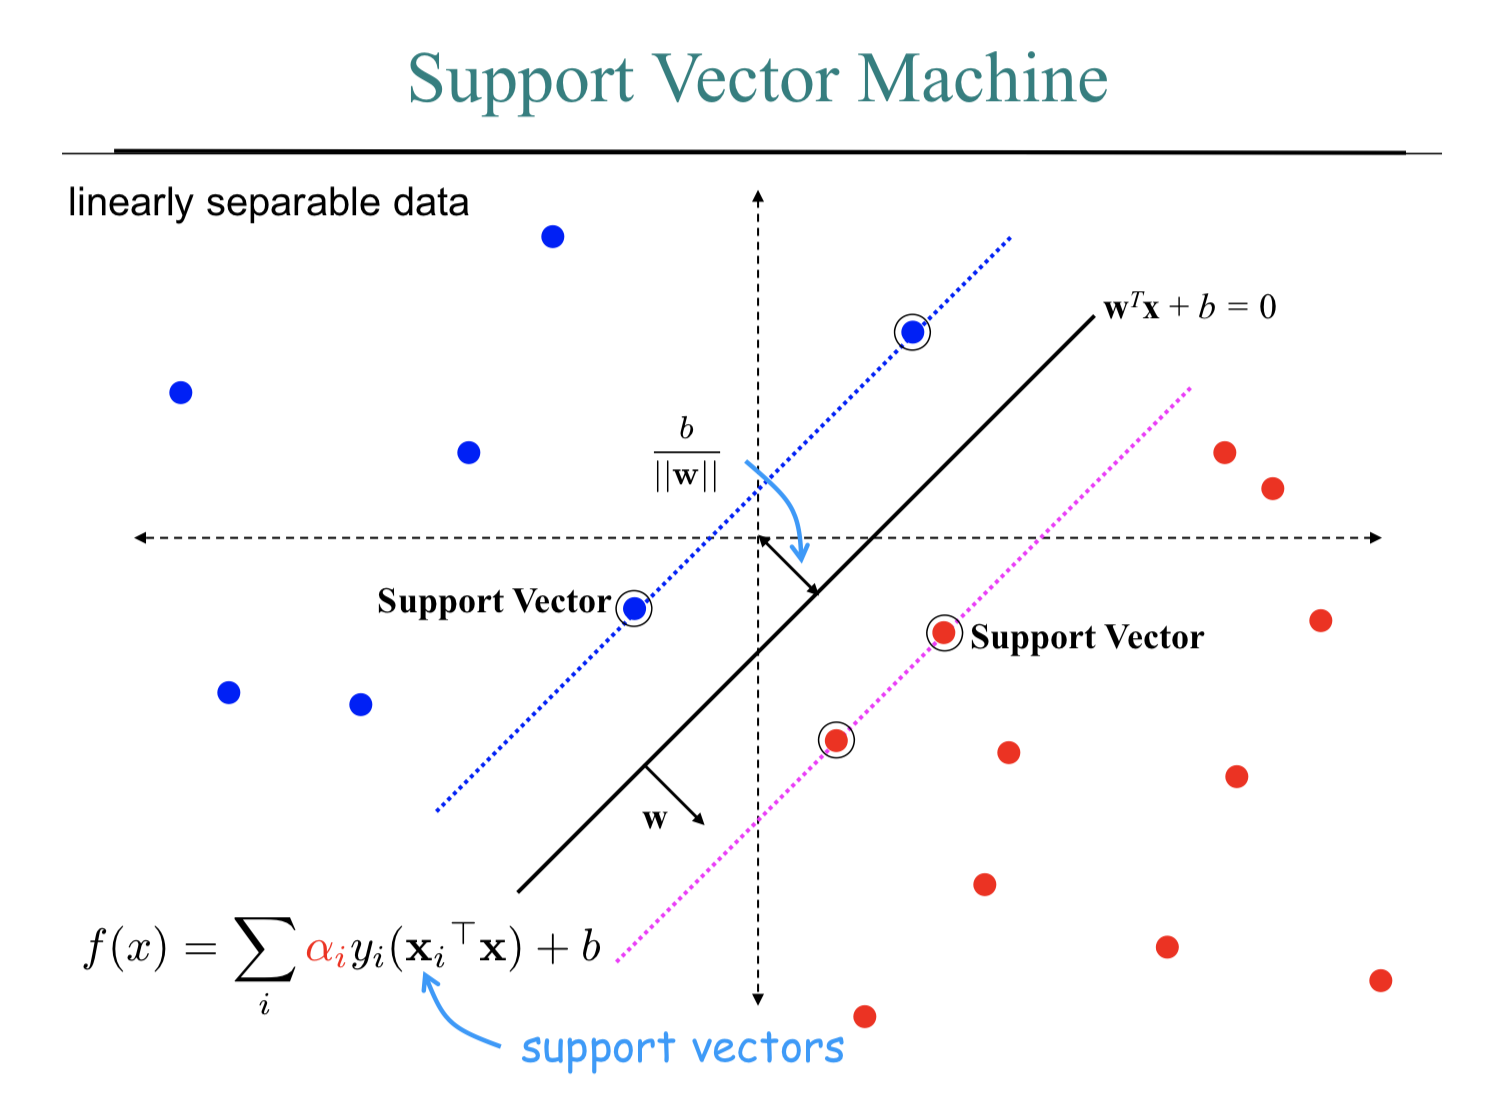
\includegraphics[width=0.9\textwidth]{img/svm_pic.png}
\caption{SVM classification}
\end{figure}

\subsection{Hard margin}
The simplest flavour of the linear SVM is referred to as the `hard magin'. In this setting, the hyperplane is chosen to maximise the distance between the nearest datasets.

Let $\mathbf{x}^+$ and $\mathbf{x}^-$ be two of the possible support vectors from each class. From the definition of the decision boundary, there is a degree of freedom in the scale of the weights $\mathbf{w}$. As a result, we normalise the weights to ensure 
\begin{align}
\mathbf{w}^\top\mathbf{x}^+=+1\\
\mathbf{w}^\top\mathbf{x}^-=-1
\end{align}
Having performed this normalisation, the length of the margin, $M$, can then be expressed in terms of the norm of the weights
\begin{align}
M &=\hat{\mathbf{w}}^\top(\mathbf{x}^+-\mathbf{x}^-)\\
&=\frac{\mathbf{w}^\top(\mathbf{x}^+-\mathbf{x}^-)}{|\mathbf{w}|}\\
&=\frac{2}{|\mathbf{w}|}
\end{align}
where $\hat{x}$ denotes the vector $x$ with unit length. As a result, maximising the margin $M$ is equivalent to the following optimisation
\begin{align}
\mathbf{w}^*=\arg\min_\mathbf{w} |\mathbf{w}|\qquad s.t. \qquad y_i(\mathbf{w}^\top\mathbf{x}_i+b)\ge1
\end{align}


\subsection{Soft margin}
When data is not linearly separable it can often be more beneficial to allow points from each class to encroach on the margin. In some cases this may mean the training points are such that the resulting hyperplane correctly classifies them (though they are closer to the hyperplane than the support vectors) though in other cases it may mean the fitted hyperplane would misclassify one or more points in the training set. The number of misclassifications will be seen to depend on a hyperparameter of the algorithm.

Figure \ref{fig:svm_slack} provides an example of binary classification where some subset of the training data is allowed to be closer to the decision boundary than the support vectors used to define it. In such a a setting, where training data enters into the margin, `slack variables' $\xi_i$ are introduced to measure how far into the margin each violation is. 

For the weights normalised as above, then the width of the margin is by definition equal to $\frac{2}{|\mathbf{w}|}$. As a result, for $\xi_i \in [0,1]$ the training point $\mathbf{x}_i$ is correctly classified though violating the margin boundary and for $\xi_i>1$ the point is misclassified. In this regard, `large' values of the slack variables constitute either more margin violations or more misclassifications. 

Capturing this in an optimisation, for some regularisation parameter $C$ we are able to formalise this as
\begin{align}
\mathbf{w}^*=\arg\min_\mathbf{w} |\mathbf{w} |+ C\sum_{i=1}^N\xi_i\\
 s.t. \qquad y_i(\mathbf{w}^\top\mathbf{x}_i+b)\ge1-\xi_i
\end{align}
where large $C$ implies heavier penalisation of the slack variables and so a `harder' margin.

Equivalently, the above optimisation may be restated in terms of the more familiar expression for $\varphi$-risk

\begin{align}
\mathbf{w}^*=\arg\min_\mathbf{w} |\mathbf{w} |+ C\sum_{i=1}^N\max(0,1-y_if(\mathbf{x}_i))
\end{align}

Note, in particular that the implied cost function can be differentiated w.r.t. each component of $\mathbf{w}$ except at discontinuities implied by the hinge loss.

\begin{figure}
\center
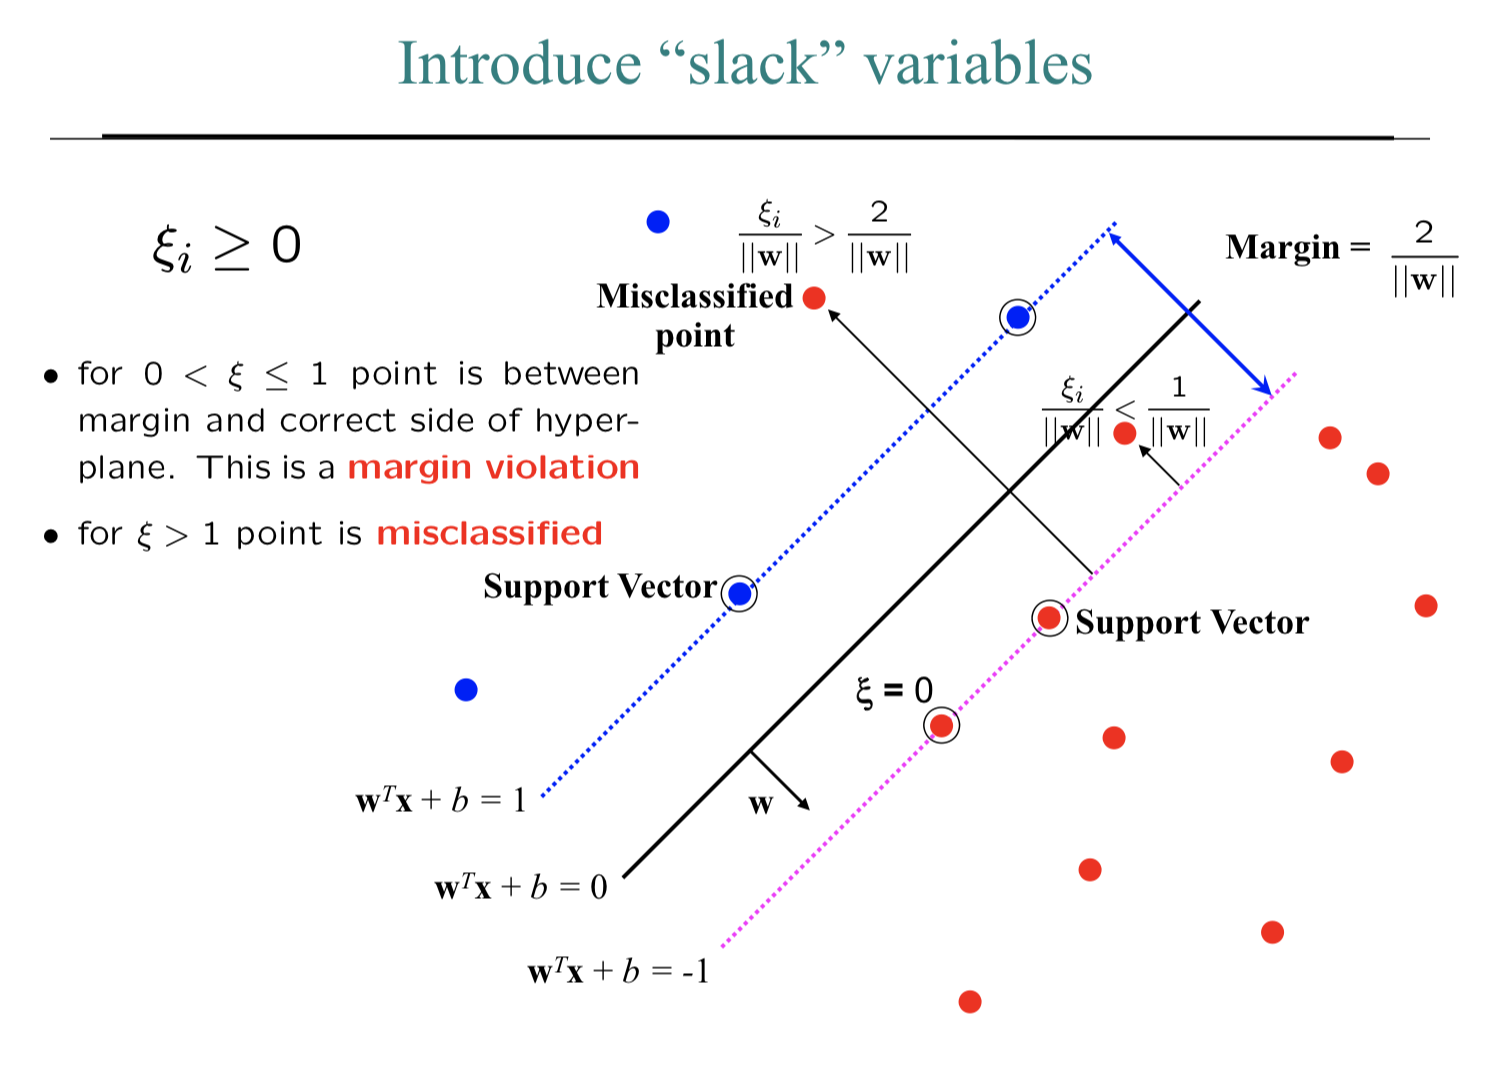
\includegraphics[width=0.9\textwidth]{img/slack_var.png}
\caption{SVM classification with slack variables}
\label{fig:svm_slack}
\end{figure}
%\subsection{Dual formulation and the `kernel trick'}


%\input{11_Kernels_SVM_written_by_Lawrence}

\section{Reproducing Kernel Hilbert Spaces}

Motivated by the above introduction to SVMs under linear classifiers, the following will extend this to the case where linear separation of the data will not yield a strong classifier. The solution to this problem can be found by introducing feature maps $\Phi\colon \mathcal{X} \rightarrow \mathcal{H}$, where $\mathcal{H}$ is an appropriate Hilbert space. With the right choice of $\mathcal{H}$ the features $\Phi(x_i), i=1, \ldots, n$ can then be separated using support vector machines. We will conclude with a coverage of generalisation bounds, aiming to analyse the trade-off between overfitting a flexible class of functions to a small amount of data and underfitting a smaller class of functions to a larger amount of data. 

As will be seen, the choice of Hilbert space used for the classification problem can be constructed through the definition of positive semi-definite kernel (defined explicitly below).  The following defines such kernels and explore some of its properties. Subsequently the construction of the relevant Hilbert space over which the classification problem for SVMs can be performed is constructed. 

\begin{definition}
A function $k\colon \mathcal{X}\times \mathcal{X} \rightarrow \mathbb{R}$ is called a \emph{positive symmetric definite kernel} (PSD kernel) if 
\begin{itemize}
	\item[i)] For all $x, y$, $$k(x, y)=k(y, x);$$
	\item[ii)] For any finite collection $x_1, \ldots, x_n \in \mathcal{X}$, the matrix defined by
	\begin{equation}
		\mathbf{K} := (k_{i,j})_{i,j} := (k(x_i, x_j))_{i,j}
	\end{equation}
	is positive \underline{semi}-definite, that is, for all $n\in \mathbb{N}$, all $x_1, \ldots, x_n$ and any $a_1, \ldots, a_n \in \mathbb{R}$ 
	\begin{equation*}
	 \sum_{i=1}^n\sum_{j=1}^n a_ia_j k(x_i, x_j) = a^T\mathbf{K}a \geq 0.
	\end{equation*}
\end{itemize}
\end{definition}

\begin{example}[Kernels]
\begin{itemize}
	\item[a)] Let $\X = \R^d$ and $k(x,y) = x^Ty$ the usual inner product. Then $k$ is a PSD since for any $a_1, \ldots, a_n \in \R$
	\begin{equation*}
		\sum_{i,j} a_ia_j x_i^Tx_j = \sum_{i,j} (a_ix_i)^T(a_j x_j) = (\sum_i a_ix_i)^T(\sum_j a_j x_j) = \left\|\sum_i a_i x_i \right\|^2 \geq 0.
	\end{equation*}
	\item[b)] \emph{(Without proof)} The Gaussian kernel (or Gaussian RBF) $$k(x, y) =  \exp\left(-\frac{\|x - y\|^2}{\gamma}\right).$$ 	
	The Gaussian kernel is governed by some parameter $\gamma >0$, which can be interpreted in the following way: consider the feature map $\Phi \colon x \mapsto k(\cdot, x)$ for some observations $x_1, \ldots, x_n$. For $\gamma$ small the features $\Phi(x_1),\ldots, \Phi(x_n)$ are almost independent, whereas for $\gamma$ large the features are almost parallel. 
\end{itemize}
\end{example}

\begin{definition}
Let $W$ denote a Hilbert space of real valued functions $f\colon \mathcal{X} \rightarrow \mathbb{R}$. A function $k\colon \mathcal{X}\times \mathcal{X} \rightarrow \mathbb{R}$ is called a \emph{reproducing kernel} for $W$ if
\begin{itemize}
	\item[i)] For all $x \in \mathcal{X}$: $k(x, \cdot) \in W$;
	\item[ii)] for all $x \in \mathcal{X}$ and $f \in W$:
	\begin{equation*}
		f(x) = \langle f, k(x, \cdot) \rangle_W \quad \text{(reproduction).}
	\end{equation*}
\end{itemize}
Hilbert spaces for which such a $k$ exists are called \emph{reproducing kernel Hilbert spaces (RKHS).}
\end{definition}
In the literature RKHS are sometimes defined as a Hilbert space of real valued functions with the property that the point evaluation functions $\delta_x \colon  f \mapsto f(x)$ are continuous for all $x \in \X$. It is not difficult--using Cauchy-Schwarz and the Riesz representation theorem--to establish that both definitions are equivalent. In fact, the continuity of evaluation functions in reproducing kernel Hilbert spaces follows from the following lemma.
\begin{lemma}\label{lem:kernel}
A kernel $k$ has the following properties 
\begin{align*}
	\langle k(x, \cdot), k(y, \cdot) \rangle_W = k(x, y)
	\intertext{and}
	\sup_{x\in{\mathcal{X}}} |f(x)| \leq \|f\|_W \sup_{x\in\mathcal{X}} \sqrt{k(x, x)}.
\end{align*}
\end{lemma}

\begin{proof}
The first part follows from reproduction 
\begin{equation*}
	\langle f, k(x, \cdot) \rangle_W = f(x) 
\end{equation*}
using $f(x) = k(y, x)$. Also by reproduction and Cauchy-Schwarz
\begin{align*}
	\sup_{x\in\X} f(x)^2 = \sup_{x\in\X} \langle f, k(x, \cdot) \rangle_W^2 \leq \sup_{x\in\X}\|f\|_W^2\|k(x, \cdot\|_W^2.
\end{align*}
By the first part $\|k(x, \cdot )\|_W^2 = \langle k(x, \cdot), k(x, \cdot) \rangle_W = k(x, x)$ so the result follows.
\end{proof}

Based on this lemma we can establish a further characterisation which is especially useful in practice (see Example c).
\begin{proposition}
If $k\colon \X \times \X$ is a reproducing kernel for some Hilbert space $W$, then $k$ is a PSD kernel. Conversely let $k$ be a PSD kernel then $k$ is a reproducing kernel. 
\end{proposition}
\begin{proof}
We show only the first part. Let $a_1, \ldots, a_n \in \R$, then
\begin{align*}
	\sum_{i,j} a_ia_j k(x_i, x_j) &= \sum_{i,j} a_ia_j \langle k(x_i, \cdot ), k(x_j, \cdot ) \rangle_W \\
	&= \left\langle \sum_{i} a_i  k(x_i, \cdot ), \sum_j a_jk(x_j, \cdot ) \right\rangle_W \\
	&= \left\| \sum_i a_i k(x_i, \cdot) \right\|_W^2 \geq 0.
\end{align*}
\end{proof}

The question that arises now is how to build a RHKS given a kernel. In the following we will give some examples how to build reproducing kernel Hilbert spaces from some kernel $k$.

\begin{example}[RKHS]
\begin{itemize}
	\item[a)] We start with a counter example. Consider the space $L^2([0, 1])$. Then the point evaluations $\delta_x: f \mapsto f(x)$ are not continuous, so $L^2([0, 1])$ cannot be a RKHS. (Note that elements of $L^2$ are only defined almost everywhere.)
	\item[b)] Denote $\varphi_1, \ldots, \varphi_n$ an orthonormal system in $L^2(\X)$. Then for arbitrary $a_k > 0, k \in \mathbb{N}$
	\begin{equation}
		k(x, y) := \sum_{j=1}^M a_j \varphi_j(x)\varphi_j(y)
	\end{equation}
	is a reproducing kernel for 
	\begin{equation*}
		W := \mathrm{span}\left\{\varphi_1, \ldots, \varphi_n\right\}
	\end{equation*}
	equipped with inner product 
	\begin{equation*}
		\langle f, g \rangle_W = \sum_{j=1}^M a_j^{-1} \langle f, \varphi_j \rangle_{L^2} \langle g, \varphi_j \rangle_{L^2}.
	\end{equation*}
	This follows for every $f \in W$ from
	\begin{align*}
		\langle f, k(x, \cdot ) \rangle_W &= \sum_{i=1}^n a_i^{-1} \langle f, \varphi_i \rangle_{L^2} \langle k(x, \cdot ), \varphi_i \rangle_{L^2} \\
		& = \sum_{i=1}^n a_i^{-1} \langle f, \varphi_i \rangle_{L^2} \langle \sum_{j=1}^n a_j \varphi_j(x)\varphi_j(\cdot), \varphi_i \rangle_{L^2} \\
		& = \sum_{i=1}^n a_i^{-1} \langle f, \varphi_i \rangle_{L^2} \sum_{j=1}^n a_j \varphi_j(x)\langle \varphi_j, \varphi_i \rangle_{L^2} \\
		& = \sum_{i=1}^n a_i^{-1} \langle f, \varphi_i \rangle_{L^2} \varphi_i(x) a_i \\
		& = \sum_{i=1}^n \langle f, \varphi_i \rangle_{L^2} \varphi_i(x) = f(x). \\
	\end{align*}
	Note that this construction can be extended to infinite series as long as $k(x, y)$ is well defined. Mercer's theorem here establishes a connection to self-adjoint integral operators.
	\item[c)] Given a PSD kernel, consider 
	\begin{equation*}
			W = \mathrm{span}\left\{k(x_1, \cdot), \ldots, k(x_n, \cdot)\right\}
	\end{equation*}
	for pairwise different $x_1, \ldots, x_n \in \X$. Note for $f, g \in W$ we can write
	\begin{equation*}
		f(x) = \sum_{i=1}^n a_i k(x_i, x), \quad g(x) = \sum_{i=1}^n b_i k(x_i, x).
	\end{equation*}
	$W$ is a RHKS with inner product
	\begin{equation*}
		\langle f, g \rangle_W = \sum_{i=1}^n\sum_{j=1}^n a_i b_i k(x_i, x_j) = a^T\mathbf{K}b.
	\end{equation*}
	Then					 
	\begin{equation*}
		f(x_j) = \sum_{i=1}^n a_i k(x_i, x_j) = \langle f, k(x_j, \cdot ) \rangle_W
	\end{equation*}
	This way is popular in practice since we can construct an RKHS by just using the PSD kernel $k$ and the datapoints $x_1, \ldots, x_n$. We can, for example, use the Gaussian radial kernel as introduced above. Then $W$ consists of linear combinations of Gaussian bell curves. %If we use $k(x, y) = \langle x, y \rangle_{\R^d}$ this leads to the space of
	\item[d)] (optional) Denote $W = \{f \colon [0, 1] \rightarrow \mathbb{R} : f(0) = 0, \int_0^1 f'(x)^2 dx < \infty \}$, where $f'$ is assumed to exist in the weak sense. $W$ is a RHKS with $\langle f, g \rangle_W = \langle f', g' \rangle$ and reproducing kernel $k(x, y) = \min\{x, y\}$ since 
	\begin{equation*} 
		\langle f, k(x, \cdot) \rangle_W = \int_0^1 f'(y)\frac{\partial }{\partial y} \min\{x, y\}dy = \int_0^1 f'(y)1_{\{y \leq x\}} dy = f(x).
	\end{equation*}
	$W$ is known more broadly as a \emph{Cameron-Martin-Space}, serving an important role in the analysis of stochastic processes. Here, $k(x, y) = \E\left[B_xB_y \right] = \min\{x, y\}$ is the covariance function of Brownian motion $(B_t)_{t \in [0, 1]}$. Further 
	\begin{equation*}
		\E\left[\langle f, B \rangle_W \langle g, B  \rangle_W \right] := \E\left[\int f' dB \int g' dB \right] = \langle f, g \rangle_W.
	\end{equation*}
\end{itemize}
\end{example}

\begin{theorem}[Representer Theorem]\label{theo:representer}
Let $W$ denote a RHKS with PSD $k$ and let $G$ denote an arbitrary function. Then
\begin{align*}
	\min_{f\in W, \|f|\leq \lambda} G\left(f(x_1), \ldots, G(f(x_n))\right) &= \min_{f\in V, \|f|\leq \lambda} G\left(f(x_1), \ldots, G(f(x_n))\right) 
\end{align*}
where we define
\begin{equation*}
	V := \mathrm{span}\left\{k(x_1, \cdot), \ldots, k(x_n, \cdot)\right\}.
\end{equation*}
Moreover, writing $f \in V$ as $f = f_a = \sum_{i=1}^n a_i k(x_i, \cdot), a \in \R^d$ we get
\begin{equation*}
	\min_{f\in W, \|f|\leq \lambda} G\left(f(x_1), \ldots, G(f(x_n))\right) = \min_{a\in \R^d, a^T\mathbf{K}a \leq \lambda^2} G\left(f_a(x_1), \ldots, G(f_a(x_n))\right).
\end{equation*}
\end{theorem}
\begin{proof}
Denote $V^\perp := \{x \in W : \langle u, v \rangle_W = 0 \quad \forall v \in V\}$ the orthogonal complement of $V$ in $W$. Then any $f\in W$ can be decomposed in $f = v + u$ with $v \in V$ and $u\in V^\perp$. Pythagoras yields
\begin{equation*}
	\|f\|_W^2 = \|v\|_W^2 + \|u\|_W^2.
\end{equation*}
Moreover, since by definition $k(x_i, \cdot) \in V$ for any $i$, we have
\begin{equation*}
	u(x_i) = \langle u, k(x_i, \cdot) \rangle_W = 0.
\end{equation*}
Hence, $f(x_i) = v(x_i)$ and $u$ does not contribute to the constraint
\begin{equation*}
	\min_{f\in W, \|v|^2+\|u|^2\leq \lambda^2} G\left(f(x_1), \ldots, G(f(x_n))\right) = \min_{v\in W, \|v|^2\leq \lambda^2} G\left(v(x_1), \ldots, G(v(x_n))\right).
\end{equation*}
This shows the first part. The second part can be seen as follows. Note that by restricting our search for the minimum to $f \in V$ we can write $f_a$ as $f_a = \sum_{i=1}^n a_i k(x_i, \cdot)$. Hence, 
\begin{align*}
	\|f_a\|^2 &= \langle f_a, f_a \rangle \\
						&= \left\langle \sum_{i=1}^n a_i k(x_i, \cdot),\sum_{j=1}^n a_j k(x_j, \cdot)\right\rangle \\
						&= \sum_{i=1}^n\sum_{j=1}^n a_i a_j \langle k(x_i, \cdot),k(x_j, \cdot) \rangle \\
						&= \sum_{i=1}^n\sum_{j=1}^n a_i a_j k(x_i,x_j) \\
						&= a^T\mathbf{K}a.
\end{align*}
This concludes the second part of the proof.
\end{proof}


\section{SVMs and RKHS}

We we will now apply these results to classification and support vector machines. Recall, we want to find the classifier (some $f$ in a pre-determined class of functions) that minimises the empirical $\varphi$-risk, where $\varphi$ denotes a convex relaxation of the $0-1$ loss. In the following, we will confine our attention to the popular hinge loss, $\varphi(z) = (1 + z)_+$.

\begin{definition}
Let $k$ denote a reproducing kernel and denote $W$ a RKHS. For $\lambda > 0$ set 
\begin{equation}\label{eq:svm}
	\hat{f}_\mathrm{SVM} := \argmin_{f \in W: \|f\|_W \leq \lambda} \frac{1}{n}\sum_{i = 1}^n \left(1 - Y_i f(X_i)\right)_+,
\end{equation}
where we used the hinge loss. 
\end{definition}

We can apply \autoref{theo:representer} to rewrite \eqref{eq:svm} as 
\begin{align*}
	\hat{f}_\mathrm{SVM} &= \argmin_{f \in W: \|f\|_W \leq \lambda} \frac{1}{n}\sum_{i = 1}^n \left(1 - Y_i f(X_i)\right)_+ \\
											 &= \argmin_{a \in \R^n: a^T\mathbf{K}a \leq \lambda^2} \frac{1}{n}\sum_{i = 1}^n \left(1 - Y_i \sum_{j=1}^n a_j k(X_i, X_j)\right)_+ \\
											 &= \argmin_{a \in \R^n} \left\{\frac{1}{n}\sum_{i = 1}^n \left(1 - Y_i \sum_{j=1}^n a_j k(X_i, X_j)\right)_+ + \lambda' \sum_{i=1}^n\sum_{j=1}^n a_ia_j K(X_i, X_j) \right\} 
\end{align*}
where we used Lagrange duality in the last line for some suitable $\lambda'$.

For further interpretation we can rewrite the minimization problem again 
\begin{align*}
	\left(\hat{f}_\mathrm{SVM}, \hat{\xi} \right) &= \argmin_{f \in W, \xi \in \R_{\geq 0}^n, Y_if(X_i) \geq 1 - \xi_i} \left\{\frac{1}{n}\sum_{i=1}^n \xi_i + \lambda'\|f\|_W^2\right\} \\
	&=\argmin_{a\in\R^n, \xi \in \R_{\geq 0}^n, Y_i\sum_{j=1}^n a_j k(X_i, X_j) \geq 1 - \xi_i} \left\{\frac{1}{n}\sum_{i=1}^n \xi_i + \lambda'a^T\mathbf{K}a\right\}.
\end{align*}
Now, if all $(X_i, Y_i)$ are classified correctly with at least $Y_if(X_i) \geq 1$, then $\hat{\xi} = 0$ and the we only minimize over $$a^T\mathbf{K}a = \sum_ia_i \sum_j a_j k(x_i, x_j)=\sum_i a_i f(x_i)_.$$


\section{Generalisation bounds}
The following inequality aims to provide some insight into the increase in expected empirical risk under the SVM classifier above the $\varphi$-risk, $\inf_{\|f\|_W\leq \lambda} R_\varphi(f)$.

\begin{theorem}[Expected Excess Risk]\label{eq:excess_risk}
Denote the (hard) SVM-classifier as $\hat{h}_n^\mathrm{SVM}$ based on the hinge-loss in a kernel RKHS $W$ with $\sup_{x \in \mathcal{X}} k(x, x) < \infty$. Then the following bound holds for the expected risk and some radius $\lambda> 0$
\begin{equation*}
	\E\left[R(\hat{h}_n^\mathrm{SVM})\right] \leq \inf_{\|f\|_W\leq \lambda} R_\varphi(f) + 8 \lambda\E\left[k(X, X)\right]^{1/2}n^{-1/2}
\end{equation*}
\end{theorem}

We will need the following contraction principle by Ledoux and Talagrand, which we will just state as a lemma.
\begin{lemma}[Contraction principle]\label{lemma:contraction}
For a map $\psi\colon [-1, 1] \rightarrow \R$ with $|\psi(x) - \psi(y)|\leq | x- y|$ and $\psi(0) = 0$ we have for any family of measurable function $\mathcal{G} = \{g: \mathcal{X} \times \{-1, +1\} \rightarrow [-1, 1]\}$
\begin{equation*}
	\E\left[\sup_{g\in \mathcal{G}}\left|\frac{1}{n}\sum_{i=1}^n\sigma_i\psi(g(X_i, Y_i))\right|\right] \leq 2\E\left[\sup_{g\in \mathcal{G}}\left|\frac{1}{n}\sum_{i=1}^n\sigma_ig(X_i, Y_i)\right|\right].
\end{equation*}
\end{lemma}

\begin{proof}[Proof of \autoref{eq:excess_risk}]
Denote $X, Y$ a sample from the joint data distribution $P^{X, Y}$ independent of $\hat{f}_n^\mathrm{SVM}$, i.e. independent of all random variables used for classification. For the hinge loss $\varphi(x) = \max\{0, 1 + x\}$ we get
\begin{align*}
	R(\hat{h}_n^\mathrm{SVM}) &= \mathbb{P}^{X, Y}(-Y\hat{f}_n^\mathrm{SVM}(X) > 0) \\ 
	&\leq \E^{X, Y}\left[\max\left\{0, 1- Y\hat{f}_n^\mathrm{SVM}(X) \right\} \right] \\
	& = R_\varphi(\hat{f}_n^\mathrm{SVM})
\end{align*}
We can estimate
\begin{equation*}
	R_\varphi(\hat{f}_n^\mathrm{SVM}) - \inf_{\|f\|_W \leq \lambda} \leq 2 \sup_{\|f\|_W\leq \lambda} \left|R_{\varphi,n}(f) - R_\varphi(f)\right|.
\end{equation*}
Hence the proof is complete as soon as we can show 
\begin{equation*}
	\E\left[\sup_{\|f\|_W\leq \lambda} \left|R_{\varphi,n}(f) - R_\varphi(f)\right|\right] \leq 4\lambda \sqrt{\frac{\E\left[k(X, X)\right]}{n}}.
\end{equation*}
By symmetrisation and a contraction argument we can upperbound the left-hand-side by the Rademacher complexity. To show this we introduce a \emph{ghost sample} $(X_i', Y_i'), i=1, \ldots,n$ which is an independent copy of the original sample following the same distribution. Denoting $\mathcal{D}$ the $\sigma$-algebra spanned by $(X_i, Y_i)_{i=1, \ldots, n}$ we get by Jensen's inequality 
\begin{align*}
	\E\left[\sup_{\|f\|_W\leq \lambda} \left|R_{\varphi,n}(f) - R_\varphi(f)\right|\right] &\leq \E\left[\sup_{\|f\|_W\leq \lambda} \left|\frac{1}{n}\sum_{i=1}^n\left(\varphi(-Y_if(X_i)) - \E\left[\varphi(-Y_i'f(X_i'))\right]\right)\right|\right] \\
	& \leq \E\left[\sup_{\|f\|_W\leq \lambda} \left|\frac{1}{n}\sum_{i=1}^n\left(\varphi(-Y_if(X_i)) - \E\left[\varphi(-Y_i'f(X_i'))\mid \mathcal{D}\right]\right)\right|\right] \\
	& \leq \E\left[\sup_{\|f\|_W\leq \lambda} \left|\E\left[\frac{1}{n}\sum_{i=1}^n\varphi(-Y_if(X_i)) - \varphi(-Y_i'f(X_i'))\mid \mathcal{D}\right]\right|\right] \\
	& \leq \E\left[\E\left[\sup_{\|f\|_W\leq \lambda} \left|\frac{1}{n}\sum_{i=1}^n\varphi(-Y_if(X_i)) - \varphi(-Y_i'f(X_i'))\right|\mid \mathcal{D}\right]\right].
\end{align*}
Now, $\pm(\varphi(-Y_if(X_i)) - \varphi(-Y_i'f(X_i')))$ have the same distribution, so we can replace this quantity with $\sigma_i\varphi(-Y_if(X_i)) - \varphi(-Y_i'f(X_i'))$, where $(\sigma_i)_{i\in \mathbb{N}}$ denotes the Rademacher process. We have
\begin{align*}
\E\left[\sup_{\|f\|_W\leq \lambda} \left|R_{\varphi,n}(f) - R_\varphi(f)\right|\right] &\leq \E\left[\sup_{\|f\|_W\leq \lambda} \left|\frac{1}{n}\sum_{i=1}^n\varphi(-Y_if(X_i)) - 1 + 1 - \varphi(-Y_i'f(X_i'))\right|\right] \\ 
&\leq 2\E\left[\sup_{\|f\|_W\leq \lambda} \left|\frac{1}{n}\sum_{i=1}^n\sigma_i\varphi(-Y_if(X_i)) - 1\right|\right]
\end{align*}
By noting that $\|f\|_W \leq \lambda$ we can conclude by \autoref{lem:kernel} that
$\|f\|_\infty \leq \lambda \sup_{x\in\X}k(x, x)^{1/2} =: L < \infty$ (by assumption).
Using the contraction argument by Ledoux and Talagrand \autoref{lemma:contraction} with the functions $\psi(z) = (\varphi(Lz) - 1)/L$ and $g(x, y) = -yf(x)/L \in [-1, 1]$ we get
\begin{equation*}
\E\left[\sup_{\|f\|_W\leq \lambda} \left|\frac{1}{n}\sum_{i=1}^n\sigma_i\frac{\varphi(-Y_if(X_i)) - 1}{L}\right|\right] \leq 2\E\left[\sup_{\|f\|_W\leq \lambda} \left|\frac{1}{n}\sum_{i=1}^n\sigma_i\frac{-Y_if(X_i)}{L}\right|\right].
\end{equation*}
The random variables $-Y_i\sigma_i$ are distributed as $\sigma_i$ which lets us conclude
\begin{equation*}
	\E\left[\sup_{\|f\|_W\leq \lambda} \left|R_{\varphi,n}(f) - R_\varphi(f)\right|\right] \leq 4 \E\left[\sup_{\|f\|_W\leq \lambda} \left|\frac{1}{n}\sum_{i=1}^n\sigma_if(X_i)\right|\right],
\end{equation*}
where the RHS denotes the Rademacher complexity $\mathcal{R}_n(\mathcal{F})$ of the set $\mathcal{F} = \{f \in W: \|f\|_W \leq \lambda\}$. 
We bound the Rademacher complexity by using the structure of the reproducing Hilbert space. With Cauchy-Schwarz we obtain
\begin{align*}
	\mathcal{R}_n(\mathcal{F}) &= \E \left[\sup_{f \in \mathcal{F}} \left|\frac{1}{n}\sum_{i=1}^n \sigma_i f(X_i)  \right| \right] \\
	& = \frac{1}{n}\E \left[\sup_{f \in \mathcal{F}} \left|\sum_{i=1}^n \sigma_i \langle k(X_i, \cdot), f \rangle_W  \right| \right] \\
	& = \frac{1}{n} \E \left[\sup_{f \in \mathcal{F}} \left|\left\langle\sum_{i=1}^n \sigma_i  k(X_i, \cdot), f \right\rangle_W  \right| \right] \\ 
	& \leq \frac{1}{n} \E \left[\sup_{f \in \mathcal{F}} \sqrt{\|f\|_W^2 \left\|\sum_{i=1}^n \sigma_i k(X_i, \cdot) \right\|_W^2}\right] \\ 
	& \leq \frac{\lambda}{n}\E \left[\sqrt{\sum_{i=1}^n \sigma_i\sigma_j k(X_i, X_j)}\right]. 
\end{align*}
Now with Jensen
\begin{align*}
	\E \left[\sqrt{\sum_{i=1}^n \sigma_i\sigma_j k(X_i, X_j)}\right] &\leq  \sqrt{\E \left[\sum_{i=1}^n \sigma_i\sigma_j k(X_i, X_j)\right]} \\ 
	&\leq  \sqrt{\sum_{i=1}^n \E\left[k(X_i, X_j)\right] \E \left[\sigma_i\sigma_j \right]} \\ 
	&\leq  \sqrt{\sum_{i=1}^n\sum_{j=1}^n\E\left[k(X_i, X_i)\right] \delta_{ij}} \\
	&\leq \sqrt{n}\sqrt{\E\left[k(X, X)\right]}.
\end{align*}
This concludes the proof.
\end{proof}
As stated, the above theorem provides only the excess risk in expectation over the data. Further (and structurally similar) bounds exist bounding the excess risk in high probability. These can be found in the Rigolet lecture notes. 
